\documentclass[12pt, a4paper]{article}

%% ── Geometry ────────────────────────────────────────────────────────────────
\usepackage[a4paper, top=2.5cm, bottom=2.5cm,
            left=2.8cm, right=2.8cm, headheight=25pt]{geometry}

%% ── Fonts ───────────────────────────────────────────────────────────────────
\usepackage[T1]{fontenc}
\usepackage[utf8]{inputenc}
\usepackage{palatino}
\usepackage{mathpazo}
\usepackage{microtype}

%% ── Mathematics ─────────────────────────────────────────────────────────────
\usepackage{amsmath, amssymb, amsthm, mathtools}
\usepackage{cancel}

%% ── Graphics & colour ───────────────────────────────────────────────────────
\usepackage{xcolor}
\usepackage{tikz}
\usetikzlibrary{arrows.meta, positioning, calc,
                decorations.pathreplacing, backgrounds, patterns}
\usepackage{pgfplots}
\pgfplotsset{compat=1.15}
\usepgfplotslibrary{fillbetween}

%% ── Tables ──────────────────────────────────────────────────────────────────
\usepackage{booktabs, array, colortbl, multirow, tabularx}
\renewcommand{\arraystretch}{1.45}

%% ── Lists ───────────────────────────────────────────────────────────────────
\usepackage{enumitem}
\setlist[itemize]{leftmargin=1.8em, itemsep=3pt, topsep=4pt}
\setlist[enumerate]{leftmargin=1.8em, itemsep=3pt, topsep=4pt}

%% ── Boxes ───────────────────────────────────────────────────────────────────
\usepackage[most]{tcolorbox}
\tcbuselibrary{skins, breakable, theorems}

%% ── Headers / footers / TOC ─────────────────────────────────────────────────
\usepackage{fancyhdr}
\usepackage{lastpage}
\usepackage{tocloft}
\usepackage{caption}
\usepackage{float}

%% ── Hyperlinks ──────────────────────────────────────────────────────────────
\usepackage[colorlinks=true, linkcolor=dkblue,
            urlcolor=dkblue, citecolor=dkblue]{hyperref}

%% ── Spacing ─────────────────────────────────────────────────────────────────
\usepackage{parskip}
\setlength{\parskip}{6pt}
\setlength{\parindent}{0pt}

%% ═══════════════════════════════════════════════════════════════════════════
%%  COLOUR PALETTE
%% ═══════════════════════════════════════════════════════════════════════════
\definecolor{dkblue}{RGB}{10, 42, 112}
\definecolor{ltblue}{RGB}{228, 236, 252}
\definecolor{amber}{RGB}{172, 118, 6}
\definecolor{ltamber}{RGB}{255, 248, 215}
\definecolor{emerald}{RGB}{6, 106, 76}
\definecolor{ltemerald}{RGB}{218, 250, 238}
\definecolor{crimson}{RGB}{148, 18, 28}
\definecolor{ltcrimson}{RGB}{255, 233, 233}
\definecolor{purple}{RGB}{82, 24, 138}
\definecolor{ltpurple}{RGB}{244, 235, 255}
\definecolor{solgreen}{RGB}{8, 90, 46}
\definecolor{ltsol}{RGB}{224, 252, 234}
\definecolor{charcoal}{RGB}{36, 36, 36}
\definecolor{slate}{RGB}{72, 84, 100}
\definecolor{tabhead}{RGB}{10, 42, 112}
\definecolor{tabeven}{RGB}{228, 236, 252}
\definecolor{orange}{RGB}{190, 85, 8}
\definecolor{ltorange}{RGB}{255, 242, 220}
\definecolor{teal}{RGB}{8, 108, 114}
\definecolor{ltteal}{RGB}{218, 248, 250}

%% ═══════════════════════════════════════════════════════════════════════════
%%  TCOLORBOX ENVIRONMENTS
%% ═══════════════════════════════════════════════════════════════════════════
\newtcolorbox{defbox}[1]{breakable,enhanced,
  colback=ltblue,colframe=dkblue,coltitle=white,
  fonttitle=\bfseries\sffamily,title={Definition\quad#1},
  arc=4pt,boxrule=1pt,left=8pt,right=8pt,top=6pt,bottom=6pt,
  attach boxed title to top left={yshift=-2mm,xshift=6mm},
  boxed title style={colback=dkblue,arc=3pt,boxrule=0pt}}

\newtcolorbox{thmbox}[1]{breakable,enhanced,
  colback=ltemerald,colframe=emerald,coltitle=white,
  fonttitle=\bfseries\sffamily,title={Theorem\quad#1},
  arc=4pt,boxrule=1pt,left=8pt,right=8pt,top=6pt,bottom=6pt,
  attach boxed title to top left={yshift=-2mm,xshift=6mm},
  boxed title style={colback=emerald,arc=3pt,boxrule=0pt}}

\newtcolorbox{propbox}[1]{breakable,enhanced,
  colback=ltemerald,colframe=emerald,coltitle=white,
  fonttitle=\bfseries\sffamily,title={Proposition\quad#1},
  arc=4pt,boxrule=1pt,left=8pt,right=8pt,top=6pt,bottom=6pt,
  attach boxed title to top left={yshift=-2mm,xshift=6mm},
  boxed title style={colback=emerald,arc=3pt,boxrule=0pt}}

\newtcolorbox{keybox}[1]{breakable,enhanced,
  colback=ltamber,colframe=amber,coltitle=white,
  fonttitle=\bfseries\sffamily,title={#1},
  arc=4pt,boxrule=1pt,left=8pt,right=8pt,top=6pt,bottom=6pt,
  attach boxed title to top left={yshift=-2mm,xshift=6mm},
  boxed title style={colback=amber,arc=3pt,boxrule=0pt}}

\newtcolorbox{exbox}[1]{breakable,enhanced,
  colback=ltpurple,colframe=purple,coltitle=white,
  fonttitle=\bfseries\sffamily,title={Worked Example\quad#1},
  arc=4pt,boxrule=1pt,left=8pt,right=8pt,top=6pt,bottom=6pt,
  attach boxed title to top left={yshift=-2mm,xshift=6mm},
  boxed title style={colback=purple,arc=3pt,boxrule=0pt}}

\newtcolorbox{warnbox}[1]{breakable,enhanced,
  colback=ltcrimson,colframe=crimson,coltitle=white,
  fonttitle=\bfseries\sffamily,title={#1},
  arc=4pt,boxrule=1pt,left=8pt,right=8pt,top=6pt,bottom=6pt,
  attach boxed title to top left={yshift=-2mm,xshift=6mm},
  boxed title style={colback=crimson,arc=3pt,boxrule=0pt}}

\newtcolorbox{notebox}[1]{breakable,enhanced,
  colback=ltorange,colframe=orange,coltitle=white,
  fonttitle=\bfseries\sffamily,title={#1},
  arc=4pt,boxrule=1pt,left=8pt,right=8pt,top=6pt,bottom=6pt,
  attach boxed title to top left={yshift=-2mm,xshift=6mm},
  boxed title style={colback=orange,arc=3pt,boxrule=0pt}}

\newtcolorbox{dynbox}[1]{breakable,enhanced,
  colback=ltteal,colframe=teal,coltitle=white,
  fonttitle=\bfseries\sffamily,title={#1},
  arc=4pt,boxrule=1pt,left=8pt,right=8pt,top=6pt,bottom=6pt,
  attach boxed title to top left={yshift=-2mm,xshift=6mm},
  boxed title style={colback=teal,arc=3pt,boxrule=0pt}}

\newtcolorbox{solbox}{breakable,enhanced,
  colback=ltsol,colframe=solgreen,coltitle=white,
  fonttitle=\bfseries\sffamily,title={Solution},
  arc=4pt,boxrule=1pt,left=8pt,right=8pt,top=6pt,bottom=6pt,
  attach boxed title to top left={yshift=-2mm,xshift=6mm},
  boxed title style={colback=solgreen,arc=3pt,boxrule=0pt}}

%% ── Theorem-style ────────────────────────────────────────────────────────────
\theoremstyle{definition}
\newtheorem{remark}{Remark}[section]

%% ═══════════════════════════════════════════════════════════════════════════
%%  MATHS MACROS
%% ═══════════════════════════════════════════════════════════════════════════
\newcommand{\R}{\mathbb{R}}
\newcommand{\dd}[1]{\,d#1}
\newcommand{\ddd}[2]{\dfrac{d#1}{d#2}}
\newcommand{\dddd}[2]{\dfrac{d^{2}#1}{d#2^{2}}}
\newcommand{\pp}[2]{\dfrac{\partial #1}{\partial #2}}
\newcommand{\eval}[2]{\left.#1\right|_{#2}}
\newcommand{\abs}[1]{\left|#1\right|}
\newcommand{\e}{\mathrm{e}}
\newcommand{\CS}{\text{CS}}
\newcommand{\PS}{\text{PS}}
\newcommand{\st}{\;\text{s.t.}\;}
\DeclareMathOperator{\sgn}{sgn}

%% ═══════════════════════════════════════════════════════════════════════════
%%  PAGE STYLE
%% ═══════════════════════════════════════════════════════════════════════════
\pagestyle{fancy}\fancyhf{}
\fancyhead[L]{\textcolor{dkblue}{\textbf{ECON 320}}
  \textcolor{slate}{ --- Integration and Economic Dynamics}}
\fancyfoot[C]{\textcolor{slate}{\small Page \thepage\ of \pageref{LastPage}}}
\renewcommand{\headrulewidth}{1.2pt}
\renewcommand{\headrule}{%
  \hbox to\headwidth{\color{dkblue}\leaders\hrule height\headrulewidth\hfill}}
\renewcommand{\footrulewidth}{0.4pt}

\renewcommand{\cftsecfont}{\bfseries\color{dkblue}}
\renewcommand{\cftsecpagefont}{\bfseries\color{dkblue}}
\renewcommand{\cftsubsecfont}{\color{charcoal}}
\setlength{\cftbeforesecskip}{4pt}

%% ═══════════════════════════════════════════════════════════════════════════
\begin{document}
%% ═══════════════════════════════════════════════════════════════════════════

%% ── COVER ───────────────────────────────────────────────────────────────────
\thispagestyle{empty}
\begin{tikzpicture}[remember picture,overlay]
  \fill[dkblue] (current page.north west)
    rectangle ([yshift=-6.2cm] current page.north east);
  \fill[amber]  ([yshift=-6.2cm] current page.north west)
    rectangle ([yshift=-6.65cm] current page.north east);
\end{tikzpicture}

\vspace*{-1.7cm}
\begin{center}
  {\color{white}\large\bfseries\sffamily ECON 320 --- Mathematical Economics}\\[10pt]
  {\color{white}\Huge\bfseries Integration and}\\[6pt]
  {\color{white}\Huge\bfseries Economic Dynamics}\\[10pt]
  {\color{amber}\Large\itshape
Fall 2026}
\end{center}

\vspace{3.8cm}
\begin{center}
\begin{tabular}{r l}
  \textbf{\textcolor{dkblue}{Instructor}}
    & Dr. Muhebullah Karimzada \\[3pt]
  \textbf{\textcolor{dkblue}{Primary Text}}
    & A.\ C.\ Chiang \& K.\ Wainwright, \textit{Fundamental Methods of}\\
    & \textit{Mathematical Economics}, 4th ed., McGraw-Hill, 2005.\\[3pt]
  \textbf{\textcolor{dkblue}{Supplementary}}
    & Hoy et al., \textit{Mathematics for Economics}, 3rd ed., MIT Press, 2011.\\[2pt]
    & Simon \& Blume, \textit{Mathematics for Economists}, Norton, 1994.\\[3pt]
  \textbf{\textcolor{dkblue}{Topics}}
    & Indefinite and definite integrals, rules of integration,\\
    & improper integrals, consumer and producer surplus,\\
    & present value of income streams, first-order differential\\
    & equations, phase diagrams, stability analysis, the Solow\\
    & growth model, first-order difference equations.\\
\end{tabular}
\end{center}

\newpage\tableofcontents\newpage

%% ═══════════════════════════════════════════════════════════════════════════
\section{Introduction: Integration as Accumulation}
%% ═══════════════════════════════════════════════════════════════════════════

Differentiation measures \emph{rates of change}; integration measures
\emph{accumulation}. These two operations are inverse to each other ---
a relationship made precise by the Fundamental Theorem of Calculus.

In economics, integration arises in three distinct but related contexts:

\begin{itemize}
  \item \textbf{Area under a curve}: Consumer surplus, producer surplus,
        deadweight loss, and the Lorenz curve all involve areas under or
        between curves.
  \item \textbf{Aggregation over time}: Present values of continuous income
        streams, total capital accumulation, and cumulative production are
        integrals over time.
  \item \textbf{Solving differential equations}: Dynamic models --- the Solow
        growth model, the Ramsey--Cass--Koopmans model, price adjustment
        dynamics --- require integrating differential equations to obtain
        time paths.
\end{itemize}

Economic \emph{dynamics} studies how endogenous variables evolve over
\emph{time} in response to shocks, policies, or intrinsic forces. Static
analysis answers ``what is the equilibrium?''; dynamic analysis answers
``how does the economy get there, and will it arrive?''

%% ═══════════════════════════════════════════════════════════════════════════
\section{The Indefinite Integral}
%% ═══════════════════════════════════════════════════════════════════════════

\subsection{Definition and Antiderivatives}

\begin{defbox}{Indefinite Integral (Antiderivative)}
A function $F(x)$ is an \textbf{antiderivative} of $f(x)$ on an interval if
$F'(x) = f(x)$ for all $x$ in that interval.

The \textbf{indefinite integral} of $f(x)$ is the family of all
antiderivatives:
\[
  \int f(x)\dd{x} = F(x) + C
\]
where $C \in \R$ is an arbitrary constant of integration.
The function $f(x)$ is called the \textbf{integrand}.
\end{defbox}

Since any two antiderivatives differ by a constant, the indefinite integral
represents a \emph{family} of functions. The constant $C$ is determined by an
\textbf{initial condition} --- a known value of $F$ at some point.
\newpage
\subsection{Basic Integration Rules}

\begin{thmbox}{Standard Integration Formulae}
Let $f$ and $g$ be integrable and $a, n$ be constants ($n \neq -1$):
\begin{align}
  \int x^n \dd{x} &= \frac{x^{n+1}}{n+1} + C \tag{Power Rule} \\[4pt]
  \int \frac{1}{x}\dd{x} &= \ln|x| + C \tag{Reciprocal} \\[4pt]
  \int e^{ax}\dd{x} &= \frac{1}{a}e^{ax} + C \tag{Exponential} \\[4pt]
  \int a^x\dd{x} &= \frac{a^x}{\ln a} + C,\quad a>0,\,a\neq 1 \tag{General Exp.} \\[4pt]
  \int [af(x) + bg(x)]\dd{x} &= a\!\int f(x)\dd{x} + b\!\int g(x)\dd{x} \tag{Linearity} \\[4pt]
  \int e^x\dd{x} &= e^x + C \tag{Natural Exp.} \\[4pt]
  \int \ln x\dd{x} &= x\ln x - x + C,\quad x>0 \tag{Natural Log}
\end{align}
\emph{(Chiang \& Wainwright, p.\ 407; Simon \& Blume, pp.\ 540--545)}
\end{thmbox}

\begin{exbox}{Applying the Basic Rules}
\textbf{1.} $\displaystyle\int (3x^4 - 5x^2 + 7x - 2)\dd{x}
= \frac{3x^5}{5} - \frac{5x^3}{3} + \frac{7x^2}{2} - 2x + C$

\textbf{2.} $\displaystyle\int \frac{4}{x^3}\dd{x}
= 4\int x^{-3}\dd{x} = 4\cdot\frac{x^{-2}}{-2} + C = -\frac{2}{x^2} + C$

\textbf{3.} Find $TC(Q)$ given $MC(Q) = 3Q^2 - 8Q + 5$ and $TC(0) = 100$ (fixed cost):
\[
  TC(Q) = \int (3Q^2 - 8Q + 5)\dd{Q} = Q^3 - 4Q^2 + 5Q + C
\]
Applying $TC(0) = 100$: $C = 100$. So $TC(Q) = Q^3 - 4Q^2 + 5Q + 100$.

\textbf{4. Economic interpretation}: $K(t) = \int I(t)\dd{t}$ --- the capital
stock at time $t$ is the cumulative integral of investment flows. If
$I(t) = I_0 e^{gt}$, then $K(t) = (I_0/g)e^{gt} + C$, and the constant $C$
is determined by the initial capital stock $K(0) = K_0$.
\end{exbox}

\subsection{Techniques of Integration}

\subsubsection*{Integration by Substitution}

\begin{thmbox}{Substitution Rule}
If $u = g(x)$ is differentiable and $f$ is continuous, then:
\[
  \int f(g(x))\,g'(x)\dd{x} = \int f(u)\dd{u}
\]
\emph{Procedure}: identify an inner function $u=g(x)$, compute $du=g'(x)\,dx$,
substitute, integrate in $u$, substitute back.
\end{thmbox}

\begin{exbox}{Substitution}
\textbf{1.} $\displaystyle\int 2x(x^2+3)^5\dd{x}$:

Let $u = x^2+3$, $du = 2x\,dx$:
$\displaystyle\int u^5\dd{u} = \frac{u^6}{6} + C = \frac{(x^2+3)^6}{6} + C$

\textbf{2.} $\displaystyle\int \frac{e^{\sqrt{x}}}{\sqrt{x}}\dd{x}$:

Let $u=\sqrt{x}$, $du = dx/(2\sqrt{x})$, so $dx/\sqrt{x} = 2\,du$:
$\displaystyle\int e^u\cdot 2\dd{u} = 2e^u + C = 2e^{\sqrt{x}} + C$

\textbf{3.} $\displaystyle\int \frac{x}{x^2+1}\dd{x}$:

Let $u=x^2+1$, $du=2x\,dx$:
$\displaystyle\frac{1}{2}\int\frac{du}{u} = \frac{1}{2}\ln(x^2+1) + C$
\end{exbox}

\subsubsection*{Integration by Parts}

\begin{thmbox}{Integration by Parts}
\[
  \int u\,dv = uv - \int v\,du
\]
Choose $u$ and $dv$ so that $\int v\,du$ is easier than the original.
A useful mnemonic for choosing $u$: \textbf{LIATE} (Logarithm, Inverse trig,
Algebraic, Trig, Exponential --- choose $u$ from whichever comes first).
\emph{(Chiang \& Wainwright, p.\ 411)}
\end{thmbox}

\begin{exbox}{Integration by Parts}
\textbf{1.} $\displaystyle\int x e^x\dd{x}$:

Let $u=x$, $dv=e^x\,dx$; then $du=dx$, $v=e^x$:
\[
  \int xe^x\dd{x} = xe^x - \int e^x\dd{x} = xe^x - e^x + C = e^x(x-1) + C
\]

\textbf{2.} $\displaystyle\int x^2 e^{-x}\dd{x}$:

Apply parts twice. Let $u=x^2$, $dv=e^{-x}dx$; $du=2x\,dx$, $v=-e^{-x}$:
\[
  = -x^2 e^{-x} + 2\int xe^{-x}\dd{x}
\]
Apply parts again to $\int xe^{-x}\dd{x}$: $u=x$, $dv=e^{-x}dx$; $v=-e^{-x}$:
\[
  = -x^2 e^{-x} + 2\left[-xe^{-x} + \int e^{-x}\dd{x}\right]
  = -x^2 e^{-x} - 2xe^{-x} - 2e^{-x} + C
  = -e^{-x}(x^2+2x+2) + C
\]

\textbf{3.} $\displaystyle\int \ln x\dd{x}$:

Let $u=\ln x$, $dv=dx$; $du=dx/x$, $v=x$:
\[
  \int\ln x\dd{x} = x\ln x - \int x\cdot\frac{1}{x}\dd{x} = x\ln x - x + C
\]

\textbf{Economic application}: The present value of a linearly growing payment
$\int_0^T t\,e^{-rt}\dd{t}$ requires integration by parts twice; this is the
\emph{present value of a growing annuity}.
\end{exbox}

%% ═══════════════════════════════════════════════════════════════════════════
\section{The Definite Integral}
%% ═══════════════════════════════════════════════════════════════════════════

\subsection{Definition and the Fundamental Theorem}

\begin{defbox}{Definite Integral}
The \textbf{definite integral} of $f$ from $a$ to $b$ is:
\[
  \int_a^b f(x)\dd{x} = \lim_{n\to\infty}\sum_{i=1}^n f(x_i^*)\,\Delta x
  = F(b) - F(a)
\]
where $F$ is any antiderivative of $f$ and the limit is the Riemann sum.
Geometrically, $\int_a^b f(x)\dd{x}$ equals the \emph{net signed area}
between the curve $y=f(x)$ and the $x$-axis over $[a,b]$.
\end{defbox}

\begin{thmbox}{Fundamental Theorem of Calculus}
Let $f$ be continuous on $[a,b]$ and $F$ an antiderivative of $f$.
\begin{enumerate}
  \item \textbf{Part I} (Differentiation of integrals): If
        $G(x)=\int_a^x f(t)\dd{t}$, then $G'(x)=f(x)$.
  \item \textbf{Part II} (Evaluation): $\displaystyle\int_a^b f(x)\dd{x} = F(b)-F(a)
        \equiv \eval{F(x)}{_a^b}$.
\end{enumerate}
\emph{(Chiang \& Wainwright, p.\ 417; Simon \& Blume, p.\ 550)}
\end{thmbox}
\newpage
\begin{keybox}{Properties of the Definite Integral}
\begin{itemize}
  \item $\displaystyle\int_a^a f(x)\dd{x} = 0$
  \item $\displaystyle\int_a^b f(x)\dd{x} = -\int_b^a f(x)\dd{x}$
  \item $\displaystyle\int_a^b f(x)\dd{x} = \int_a^c f(x)\dd{x} + \int_c^b f(x)\dd{x}$ (additivity)
  \item $\displaystyle\int_a^b [af(x)+bg(x)]\dd{x} = a\!\int_a^b f\dd{x} + b\!\int_a^b g\dd{x}$ (linearity)
  \item If $f(x)\geq g(x)$ on $[a,b]$: $\displaystyle\int_a^b f\dd{x}\geq\int_a^b g\dd{x}$
\end{itemize}
\end{keybox}

\begin{center}
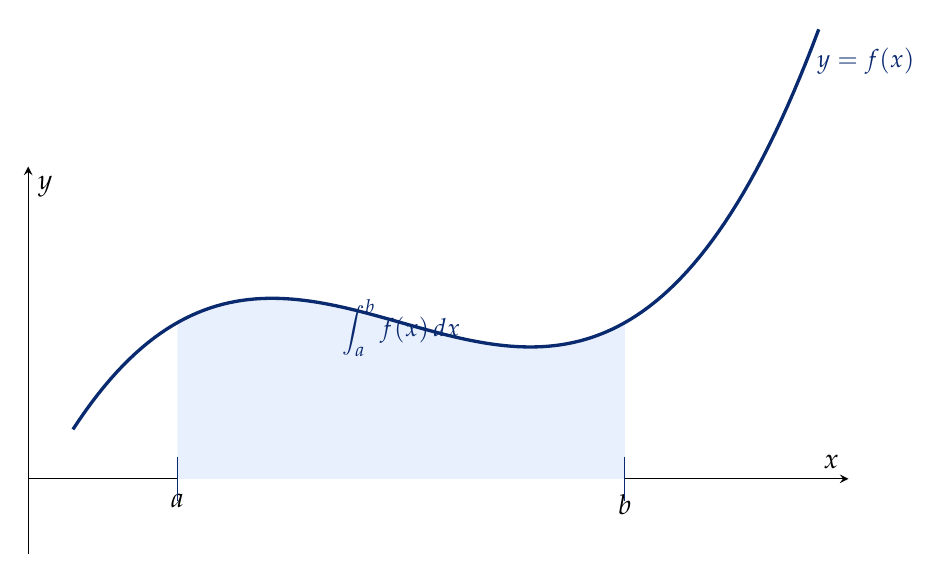
\begin{tikzpicture}
\begin{axis}[
  width=12cm, height=6.5cm,
  axis lines=center,
  xlabel={$x$}, ylabel={$y$},
  xmin=0, xmax=5.5, ymin=-1.2, ymax=5,
  xtick={1,4}, xticklabels={$a$,$b$},
  ytick=\empty, tick style={draw=none},
  grid=none, clip=false,
]
  \addplot[name path=curve, dkblue, very thick, domain=0.3:5.3, samples=120]
    {0.3*(x-1)*(x-4)*(x-2.5)+2.5} node[right,pos=0.95,font=\small]{$y=f(x)$};
  \addplot[name path=zero, draw=none, domain=1:4]{0};
  \addplot[ltblue!80] fill between[of=curve and zero, soft clip={domain=1:4}];
  \addplot[only marks, mark=|, mark size=8pt, dkblue]
    coordinates{(1,0)(4,0)};
  \node[dkblue, font=\small, above] at (axis cs:2.5,1.8){$\displaystyle\int_a^b f(x)\,dx$};
\end{axis}
\end{tikzpicture}
\captionof*{figure}{\small The definite integral equals the net signed area
between $f(x)$ and the $x$-axis over $[a,b]$.}
\end{center}

\subsection{Improper Integrals}

\begin{defbox}{Improper Integrals}
An integral is \textbf{improper} when the interval is unbounded or the
integrand has a discontinuity within the interval.

\textbf{Type I} (infinite limits):
\[
  \int_a^{\infty} f(x)\dd{x}
  = \lim_{T\to\infty}\int_a^T f(x)\dd{x}
\]
The integral \textbf{converges} if this limit is finite; otherwise it
\textbf{diverges}.

\textbf{Type II} (discontinuous integrand): similarly handled with limits.
\end{defbox}
\newpage
\begin{exbox}{Improper Integrals in Economics}
\textbf{1. Perpetuity}:
$\displaystyle\int_0^\infty Ce^{-rt}\dd{t}
= \eval{-\frac{C}{r}e^{-rt}}{_0^\infty}
= 0 - \left(-\frac{C}{r}\right)
= \frac{C}{r}$

(Requires $r>0$.) This is the present value of a constant income stream $C$
in perpetuity, discounted continuously at rate $r$.

\textbf{2. Growing perpetuity}:
$\displaystyle\int_0^\infty Ce^{gt}e^{-rt}\dd{t}
= C\int_0^\infty e^{-(r-g)t}\dd{t}
= \frac{C}{r-g}$, provided $r>g$.

This is the Gordon Growth Model in continuous time: present value of a
stream growing at rate $g$ and discounted at rate $r>g$.

\textbf{3. Divergence when $r\leq g$}:
If $r\leq g$ the integral diverges: the present value is infinite because
the income stream grows at least as fast as the discount rate.
\end{exbox}

%% ═══════════════════════════════════════════════════════════════════════════
\section{Economic Applications of Integration}
%% ═══════════════════════════════════════════════════════════════════════════

\subsection{Consumer Surplus and Producer Surplus}

\begin{defbox}{Consumer and Producer Surplus}
Let $P = D(Q)$ be the inverse demand (willingness-to-pay) and
$P = S(Q)$ be the inverse supply, with equilibrium $(Q^*,P^*)$.

\textbf{Consumer Surplus (CS)} is the area below the demand curve and
above the equilibrium price:
\[
  \CS = \int_0^{Q^*}[D(Q) - P^*]\dd{Q}
\]

\textbf{Producer Surplus (PS)} is the area above the supply curve and
below the equilibrium price:
\[
  \PS = \int_0^{Q^*}[P^* - S(Q)]\dd{Q}
\]

\textbf{Total surplus} $= \CS + \PS$. \textbf{Deadweight Loss (DWL)}
from a distortion is the reduction in total surplus.
\emph{(Chiang \& Wainwright, p.\ 421; Hoy et al., p.\ 351)}
\end{defbox}

\begin{center}
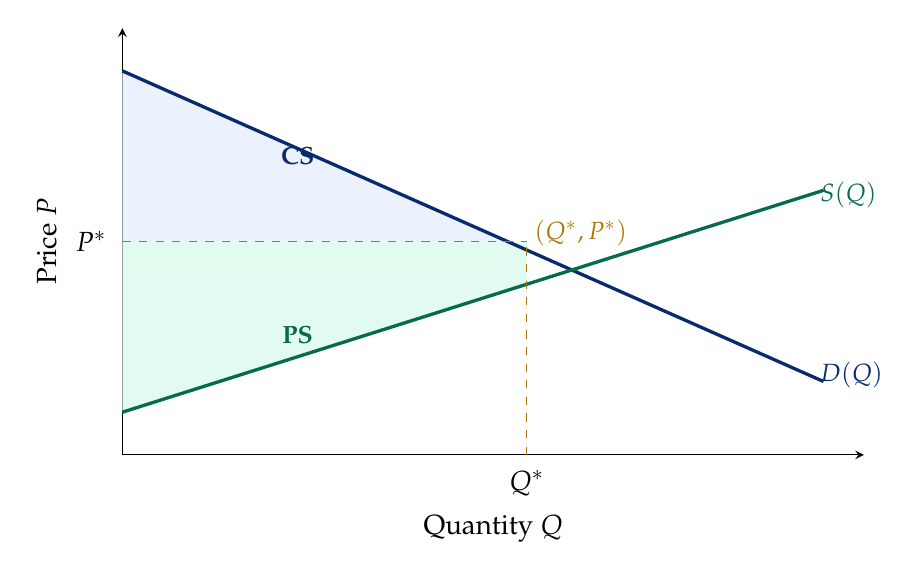
\begin{tikzpicture}
\begin{axis}[
  width=11cm, height=7cm,
  axis lines=left,
  xlabel={Quantity $Q$}, ylabel={Price $P$},
  xmin=0, xmax=5.5, ymin=0, ymax=10,
  xtick={3}, xticklabels={$Q^*$},
  ytick={5}, yticklabels={$P^*$},
  tick style={draw=none}, grid=none, clip=false,
]
  %% Demand: P = 9-Q  (linear)
  \addplot[name path=demand, dkblue, very thick, domain=0:5.2]{9-1.4*x}
    node[right,pos=0.98,font=\small]{$D(Q)$};
  %% Supply: P = 1+Q
  \addplot[name path=supply, emerald, very thick, domain=0:5.2]{1+1*x}
    node[right,pos=0.98,font=\small]{$S(Q)$};
  %% Price line
  \addplot[name path=price, amber, dashed, domain=0:3]{5};
  %% Q* vertical
  \addplot[amber, dashed, thin] coordinates{(3,0)(3,5)};

  %% CS fill (between demand and P* up to Q*)
  \addplot[name path=top_cs, dkblue, draw=none, domain=0:3]{9-1.4*x};
  \addplot[name path=bot_cs, draw=none, domain=0:3]{5};
  \addplot[ltblue!70] fill between[of=top_cs and bot_cs];

  %% PS fill (between P* and supply up to Q*)
  \addplot[name path=top_ps, draw=none, domain=0:3]{5};
  \addplot[name path=bot_ps, emerald, draw=none, domain=0:3]{1+1*x};
  \addplot[ltemerald!80] fill between[of=top_ps and bot_ps];

  \node[dkblue,font=\small\bfseries] at (axis cs:1.3,7){CS};
  \node[emerald,font=\small\bfseries] at (axis cs:1.3,2.8){PS};
  \node[amber,font=\small] at (axis cs:3.4,5.2){$(Q^*,P^*)$};
\end{axis}
\end{tikzpicture}
\captionof*{figure}{\small Consumer surplus (blue) and producer surplus
(green) at the competitive equilibrium.}
\end{center}

\begin{exbox}{Computing Consumer and Producer Surplus}
\textbf{Market:} $D(Q) = 10 - Q$ (inverse demand), $S(Q) = 2 + Q$
(inverse supply).

\textbf{Equilibrium}: $10-Q = 2+Q \Rightarrow Q^*=4$, $P^*=6$.

\textbf{Consumer Surplus:}
\[
  \CS = \int_0^4[(10-Q)-6]\dd{Q}
      = \int_0^4(4-Q)\dd{Q}
      = \eval{\left(4Q-\frac{Q^2}{2}\right)}{_0^4}
      = 16-8 = 8
\]

\textbf{Producer Surplus:}
\[
  \PS = \int_0^4[6-(2+Q)]\dd{Q}
      = \int_0^4(4-Q)\dd{Q}
      = 8
\]
Total surplus $= 16$.

\textbf{Effect of a price floor at $\bar P = 7$:}

At $\bar P=7$: $Q_d = 10-7 = 3$, $Q_s = 7-2 = 5$. Only $Q_d=3$ units
traded (demand is binding).

\[
  \CS' = \int_0^3[(10-Q)-7]\dd{Q} = \int_0^3(3-Q)\dd{Q}
       = \eval{\left(3Q-\frac{Q^2}{2}\right)}{_0^3} = 9-4.5 = 4.5
\]

\[
  \PS' = \int_0^3[7-(2+Q)]\dd{Q} = \int_0^3(5-Q)\dd{Q}
       = 15-4.5 = 10.5
\]

Total surplus $= 15$. DWL $= 16-15 = 1$.
\end{exbox}

\subsection{Present Value of Continuous Income Streams}

\begin{defbox}{Present Value of a Continuous Stream}
The \textbf{present value} at time $t=0$ of a continuous income stream
$f(t)$ over $[0,T]$, discounted at continuous rate $r$:
\[
  PV = \int_0^T f(t)\,e^{-rt}\dd{t}
\]
For a perpetual stream ($T \to \infty$):
$PV = \displaystyle\int_0^\infty f(t)\,e^{-rt}\dd{t}$, provided the integral converges.
\end{defbox}
\newpage
\begin{exbox}{Present Value Calculations}
\textbf{1. Constant stream}: $f(t)=C$, discount rate $r$, horizon $T$:
\[
  PV = \int_0^T Ce^{-rt}\dd{t}
     = \eval{-\frac{C}{r}e^{-rt}}{_0^T}
     = \frac{C}{r}(1-e^{-rT})
\]
As $T\to\infty$: $PV \to C/r$ (perpetuity formula).

\textbf{2. Growing stream}: $f(t) = Ae^{gt}$, horizon $T$, $r\neq g$:
\[
  PV = A\int_0^T e^{(g-r)t}\dd{t}
     = \frac{A}{g-r}\left(e^{(g-r)T}-1\right)
     = \frac{A}{r-g}\left(1-e^{(g-r)T}\right)
\]

\textbf{3. Investment project}: revenues $R(t)=1000e^{0.02t}$,
costs $c=400$/year, horizon $T=5$, $r=0.08$:
\[
  NPV = \int_0^5(1000e^{0.02t}-400)e^{-0.08t}\dd{t}
      = 1000\int_0^5 e^{-0.06t}\dd{t} - 400\int_0^5 e^{-0.08t}\dd{t}
\]
\[
  = \frac{1000}{0.06}(1-e^{-0.3}) - \frac{400}{0.08}(1-e^{-0.4})
  \approx 16667(0.2592) - 5000(0.3297)
  \approx 4320 - 1649 = 2671
\]
Since NPV $>0$, the project is worth undertaking.

\textbf{4. Lorenz Curve and Gini Coefficient}:
The Lorenz curve $L(s)$ gives the share of income held by the bottom
$s$ fraction of the population. The Gini coefficient is:
\[
  G = 1 - 2\int_0^1 L(s)\dd{s}
\]
If $L(s)=s^2$ (quadratic Lorenz curve):
$\int_0^1 s^2\dd{s} = 1/3$, so $G = 1-2/3 = 1/3$.
\end{exbox}

\subsection{Capital Accumulation}

\begin{exbox}{Net Investment and Capital Stock}
\textbf{Net investment} is $I(t) = \dot K(t)$ (the flow of new capital).
The capital stock at time $T$ is:
\[
  K(T) = K(0) + \int_0^T I(t)\dd{t}
\]

\textbf{Example}: $I(t) = 10\sqrt{t}$ with $K(0) = 50$:
\[
  K(T) = 50 + \int_0^T 10t^{1/2}\dd{t}
       = 50 + \eval{\frac{20t^{3/2}}{3}}{_0^T}
       = 50 + \frac{20T^{3/2}}{3}
\]
At $T=9$: $K(9) = 50 + 20(27)/3 = 50+180 = 230$.
\end{exbox}

%% ═══════════════════════════════════════════════════════════════════════════
\section{First-Order Differential Equations}
%% ═══════════════════════════════════════════════════════════════════════════

\subsection{Definitions and Classification}

\begin{defbox}{Differential Equation}
A \textbf{differential equation} is an equation involving a function and
its derivatives. A \textbf{first-order ordinary differential equation} (ODE)
has the form:
\[
  \ddd{y}{t} = f(t, y) \qquad \text{or equivalently} \quad
  F(t, y, \dot y) = 0
\]
The \textbf{general solution} contains an arbitrary constant $C$; an
\textbf{initial condition} $y(t_0)=y_0$ pins down the \textbf{particular
solution}.
\end{defbox}

\begin{defbox}{Autonomous vs.\ Non-Autonomous}
A differential equation $\dot y = f(t,y)$ is:
\begin{itemize}
  \item \textbf{Autonomous}: $\dot y = f(y)$ --- the right-hand side does not
        explicitly depend on $t$. The dynamics depend only on the current
        state, not on time itself.
  \item \textbf{Non-autonomous}: $\dot y = f(t,y)$ --- time appears explicitly.
\end{itemize}
Autonomous equations arise naturally in steady-state economic models (Solow,
Ramsey). Their phase diagrams are one-dimensional and greatly simplify
analysis.
\end{defbox}

\subsection{Linear First-Order ODEs}

\begin{thmbox}{Solution of the Linear First-Order ODE}
The \textbf{linear first-order ODE}:
\[
  \dot y + a(t)\,y = b(t)
\]
has the general solution (via the \textbf{integrating factor}
$\mu(t) = e^{\int a(t)\dd{t}}$):
\[
  y(t) = e^{-\int a(t)\dd{t}}\!\left[\int b(t)\,e^{\int a(t)\dd{t}}\dd{t} + C\right]
\]

\textbf{Constant-coefficient case} ($a(t)=a$, $b(t)=b$):
\[
  \boxed{y(t) = \underbrace{Ae^{-at}}_{\text{complementary (homogeneous)}}
               + \underbrace{\frac{b}{a}}_{\text{particular solution}}}
  \qquad A = y_0 - \frac{b}{a}
\]
The \textbf{equilibrium} (particular solution) is $y^* = b/a$; the
complementary function $Ae^{-at}$ captures departure from equilibrium.
\emph{(Chiang \& Wainwright, p.\ 468; Hoy et al., p.\ 577)}
\end{thmbox}

\begin{proof}[Derivation via Integrating Factor]
For $\dot y + ay = b$, multiply both sides by $e^{at}$:
\[
  e^{at}\dot y + ae^{at}y = be^{at}
  \iff \frac{d}{dt}\!\left[e^{at}y\right] = be^{at}
\]
Integrating both sides:
$e^{at}y = \dfrac{b}{a}e^{at} + C \Rightarrow y = \dfrac{b}{a} + Ce^{-at}$.

Applying $y(0)=y_0$: $C = y_0 - b/a = A$.
\end{proof}

\begin{keybox}{Stability of the Constant-Coefficient Linear ODE}
For $\dot y + ay = b$ with solution $y(t) = Ae^{-at} + b/a$:
\begin{itemize}
  \item \textbf{Stable} ($a>0$): as $t\to\infty$, $e^{-at}\to 0$, so
        $y(t)\to y^*=b/a$ regardless of initial conditions. The equilibrium
        is globally asymptotically stable.
  \item \textbf{Unstable} ($a<0$): $e^{-at}\to\infty$, so $y(t)$ diverges
        from $y^*$ (except from $y^*$ itself).
  \item \textbf{Neutral} ($a=0$): $y(t) = y_0 + bt$ (linear trend; no
        equilibrium unless $b=0$).
\end{itemize}
The sign of $a$ --- the coefficient of $y$ --- governs stability.
\end{keybox}

\begin{exbox}{Price Adjustment Dynamics}
Suppose the rate of price adjustment is proportional to excess demand:
\[
  \dot P = \alpha[D(P) - S(P)], \qquad \alpha > 0
\]
For linear demand and supply: $D(P) = a-bP$ and $S(P) = c+dP$:
\[
  \dot P = \alpha[(a-c) - (b+d)P]
\]
This is $\dot P + \alpha(b+d)P = \alpha(a-c)$, a linear first-order ODE with
$a_{\text{ode}} = \alpha(b+d) > 0$ and $b_{\text{ode}} = \alpha(a-c)$.

\textbf{Solution:}
$P(t) = [P(0) - P^*]e^{-\alpha(b+d)t} + P^*$, \quad where $P^* = (a-c)/(b+d)$.

Since $\alpha(b+d)>0$, the equilibrium price $P^*$ is \textbf{globally stable}:
$P(t)\to P^*$ as $t\to\infty$ from any initial condition $P(0)$.

The speed of convergence is $\alpha(b+d)$ --- faster adjustment $\alpha$,
steeper demand slope $b$, or steeper supply slope $d$ all accelerate
convergence to equilibrium.
\end{exbox}

\begin{exbox}{The Solow Growth Model}
The Solow model in intensive form (per-worker capital $k = K/L$):
\[
  \dot k = sf(k) - (n+\delta)k
\]
where $s\in(0,1)$ is the savings rate, $f(k)=k^\alpha$ is Cobb-Douglas
production per worker, $n$ is population growth, and $\delta$ is
depreciation.

This is a \textbf{nonlinear} autonomous ODE (because $f(k)=k^\alpha$ is
nonlinear). We cannot solve it in closed form for general $\alpha$. Instead:

\textbf{Steady state}: $\dot k=0 \Rightarrow sf(k^*)=(n+\delta)k^*$.
For $f(k)=k^\alpha$: $sk^{*\alpha} = (n+\delta)k^*$, giving:
\[
  k^* = \left(\frac{s}{n+\delta}\right)^{1/(1-\alpha)}
\]

\textbf{Linearisation around $k^*$}: Let $\tilde k = k - k^*$ (small deviation).
\[
  \dot{\tilde k} \approx [sf'(k^*) - (n+\delta)]\,\tilde k
\]
Stability coefficient: $\lambda = sf'(k^*) - (n+\delta) = s\alpha k^{*\alpha-1} - (n+\delta)$.

At the steady state, $sk^{*\alpha}=(n+\delta)k^*$ implies
$sk^{*\alpha-1}=(n+\delta)$. Therefore,
\[
  \lambda = s\alpha k^{*\alpha-1}-(n+\delta)
  = \alpha(n+\delta)-(n+\delta)
  = -(1-\alpha)(n+\delta) < 0.
\]

Since $\lambda < 0$ (as $\alpha \in(0,1)$ and $n+\delta>0$), the steady
state $k^*$ is \textbf{locally asymptotically stable}. Capital converges to
$k^*$ from any nearby initial condition.

\textbf{Speed of convergence}: $|\lambda| = (1-\alpha)(n+\delta)$.
For typical values $\alpha=1/3$, $n=0.01$, $\delta=0.05$:
$|\lambda| = (2/3)(0.06) = 0.04$ --- the economy closes 4\% of the gap
toward $k^*$ per year, implying a half-life of $\ln 2/0.04 \approx 17$ years.
\end{exbox}

\subsection{Separable Differential Equations}

\begin{defbox}{Separable ODE}
A first-order ODE is \textbf{separable} if it can be written as:
\[
  \frac{dy}{dt} = g(t)\,h(y)
\]
\textbf{Solution method}: separate variables and integrate:
\[
  \int \frac{dy}{h(y)} = \int g(t)\dd{t}
\]
\end{defbox}

\begin{exbox}{Separable ODEs in Economics}
\textbf{1.} Solve $\dot y = ry$ (exponential growth/decay):
\[
  \frac{dy}{y} = r\dd{t} \implies \ln|y| = rt + C_0 \implies y(t) = Ae^{rt}
\]
Initial condition $y(0)=y_0$: $A=y_0$.  So $y(t) = y_0 e^{rt}$.

\textbf{2. Logistic growth} (bounded population or market saturation):
\[
  \dot N = rN\!\left(1-\frac{N}{K}\right)
\]
Separate: $\displaystyle\int\frac{dN}{N(1-N/K)} = \int r\dd{t}$

Using partial fractions: $\displaystyle\frac{1}{N(1-N/K)} = \frac{1}{N} + \frac{1/K}{1-N/K}$:

$\ln N - \ln(1-N/K) = rt + C$

$\ln\!\dfrac{N}{1-N/K} = rt+C \Rightarrow \dfrac{N}{K-N} = Ae^{rt}$

Solving: $\boxed{N(t) = \dfrac{K}{1 + Be^{-rt}}}$, \;
$B = \dfrac{K-N_0}{N_0}$.

As $t\to\infty$: $N(t)\to K$ --- the carrying capacity.
This model fits the adoption of new technologies, market penetration, and
population dynamics.

\textbf{3. Bernoulli equation}: $\dot k = sk^\alpha - (n+\delta)k$

This is the Solow equation. With $\alpha=1/2$, let $z=k^{1/2}$,
so
\[
  \dot z=\frac{\dot k}{2k^{1/2}}
  =\frac{s\sqrt{k}-(n+\delta)k}{2\sqrt{k}}
  =\frac{s}{2}-\frac{n+\delta}{2}z.
\]
Thus, for $\alpha=1/2$, the Solow equation becomes a linear first-order
ODE in $z=\sqrt{k}$. More generally, Bernoulli equations can be linearised
by a suitable power substitution.
\end{exbox}

%% ═══════════════════════════════════════════════════════════════════════════
\section{Phase Diagrams and Stability Analysis}
%% ═══════════════════════════════════════════════════════════════════════════

\subsection{Phase Diagrams for Autonomous Equations}

For an autonomous ODE $\dot y = f(y)$, the \textbf{phase diagram} (or
phase line) plots $\dot y$ against $y$ and allows us to read off the
dynamics without solving the equation explicitly.

\begin{keybox}{Reading a Phase Diagram}
\begin{enumerate}
  \item \textbf{Equilibria (fixed points)}: where $\dot y = f(y) = 0$.
  \item \textbf{Direction of motion}:
        \begin{itemize}
          \item $f(y) > 0 \Rightarrow \dot y > 0 \Rightarrow y$ is \emph{increasing}
                $(\rightarrow)$
          \item $f(y) < 0 \Rightarrow \dot y < 0 \Rightarrow y$ is \emph{decreasing}
                $(\leftarrow)$
        \end{itemize}
  \item \textbf{Stability of equilibrium $y^*$}:
        \begin{itemize}
          \item \textbf{Stable} (attractor): arrows point \emph{toward} $y^*$
                on both sides, i.e.\ $f'(y^*)<0$.
          \item \textbf{Unstable} (repeller): arrows point \emph{away} from
                $y^*$ on both sides, i.e.\ $f'(y^*)>0$.
          \item \textbf{Semi-stable}: arrows point toward $y^*$ on one side
                only.
        \end{itemize}
\end{enumerate}
\end{keybox}

\begin{center}
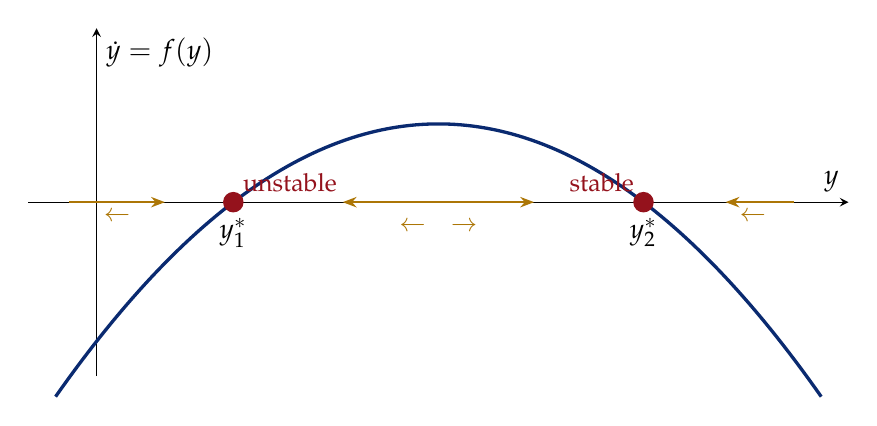
\begin{tikzpicture}
\begin{axis}[
  width=12cm, height=6cm,
  axis lines=center,
  xlabel={$y$}, ylabel={$\dot y = f(y)$},
  xmin=-0.5, xmax=5.5, ymin=-2.5, ymax=2.5,
  xtick={1,4}, xticklabels={$y_1^*$,$y_2^*$},
  ytick=\empty, tick style={draw=none},
  grid=none, clip=false,
]
  \addplot[dkblue, very thick, domain=-0.3:5.3, samples=120]
    {(x-1)*(4-x)*0.5};
  %% Equilibrium markers
  \addplot[only marks, mark=*, mark size=3.5pt, crimson] coordinates{(1,0)(4,0)};
  \node[crimson, above right, font=\small] at (axis cs:1,0){unstable};
  \node[crimson, above left, font=\small]  at (axis cs:4,0){stable};
  %% Arrows on phase line
  \draw[-{Stealth[length=5pt]},thick,amber] (axis cs:-0.2,0)--(axis cs:0.5,0);
  \draw[-{Stealth[length=5pt]},thick,amber] (axis cs:2.5,0)--(axis cs:1.8,0);
  \draw[-{Stealth[length=5pt]},thick,amber] (axis cs:2.5,0)--(axis cs:3.2,0);
  \draw[-{Stealth[length=5pt]},thick,amber] (axis cs:5.1,0)--(axis cs:4.6,0);
  \node[amber,font=\small,below] at (axis cs:0.15,0){$\leftarrow$};
  \node[amber,font=\small,below] at (axis cs:2.5,-0.15){$\leftarrow\quad\rightarrow$};
  \node[amber,font=\small,below] at (axis cs:4.8,0){$\leftarrow$};
\end{axis}
\end{tikzpicture}
\captionof*{figure}{\small Phase diagram for $\dot y=(y-y_1^*)(y_2^*-y)$.
$y_1^*$ is unstable ($f'>0$); $y_2^*$ is stable ($f'<0$).}
\end{center}

\begin{exbox}{Phase Diagram: The Solow Model}
The Solow equation $\dot k = sk^\alpha - (n+\delta)k$ defines a curve in
the $(k, \dot k)$ plane. Setting $\dot k = 0$:

\[
  sk^\alpha = (n+\delta)k \implies k^* = \left(\frac{s}{n+\delta}\right)^{1/(1-\alpha)}
\]

The slope of $\dot k$ with respect to $k$ at $k^*$:
\[
  \frac{d\dot k}{dk}\bigg|_{k^*}
  = \alpha sk^{*\alpha-1} - (n+\delta)
  = \alpha(n+\delta) - (n+\delta)
  = -(1-\alpha)(n+\delta) < 0
\]

Since the slope is negative at $k^*$, the equilibrium is \textbf{stable}.

Phase-line analysis:
\begin{itemize}
  \item For $0 < k < k^*$: $sk^\alpha > (n+\delta)k$, so $\dot k > 0$ ---
        capital per worker rises.
  \item For $k > k^*$: $sk^\alpha < (n+\delta)k$, so $\dot k < 0$ ---
        capital per worker falls.
\end{itemize}
From any $k_0 > 0$, the economy converges to $k^*$.
\end{exbox}

\subsection{Stability Conditions}

\begin{thmbox}{Local Stability via Linearisation}
For $\dot y = f(y)$ with equilibrium $f(y^*)=0$, the linearised equation
near $y^*$ is:
\[
  \dot{\tilde y} = f'(y^*)\,\tilde y, \quad \tilde y = y - y^*
\]
Solution: $\tilde y(t) = \tilde y(0)\,e^{f'(y^*)t}$.
\begin{itemize}
  \item \textbf{Locally asymptotically stable}: $f'(y^*)<0$ (eigenvalue negative).
  \item \textbf{Locally unstable}: $f'(y^*)>0$.
  \item \textbf{Non-hyperbolic} ($f'(y^*)=0$): linearisation is inconclusive.
\end{itemize}
\emph{(Chiang \& Wainwright, p.\ 475; Hoy et al., p.\ 584)}
\end{thmbox}

\begin{thmbox}{Global Stability (Lyapunov-type)}
For $\dot y = f(y)$ on $(0,\infty)$ with unique equilibrium $y^*$:
if $f(y)>0$ for $y<y^*$ and $f(y)<0$ for $y>y^*$ (phase-line arrows both
point toward $y^*$), then $y^*$ is \textbf{globally asymptotically stable}.
\end{thmbox}
\newpage
%% ═══════════════════════════════════════════════════════════════════════════
\section{First-Order Linear Difference Equations}
%% ═══════════════════════════════════════════════════════════════════════════

\subsection{Definition and Solution}

While differential equations model continuous-time dynamics, \textbf{difference
equations} model discrete-time processes.

\begin{defbox}{First-Order Linear Difference Equation}
A first-order linear difference equation with constant coefficients:
\[
  y_{t+1} = ay_t + b, \qquad t = 0, 1, 2, \ldots
\]
where $a \neq 0$ is the coefficient and $b$ is the constant term.
\end{defbox}

\begin{thmbox}{Solution of the First-Order Linear Difference Equation}
The general solution of $y_{t+1} = ay_t + b$ is:
\[
  y_t = Aa^t + y^*, \qquad y^* = \frac{b}{1-a} \; (a\neq 1)
\]
where $A = y_0 - y^*$ is determined by the initial condition $y_0$,
and $y^* = b/(1-a)$ is the \textbf{intertemporal equilibrium}.

If $a=1$: $y_t = y_0 + bt$ (linear trend, no equilibrium unless $b=0$).
\emph{(Chiang \& Wainwright, p.\ 558; Hoy et al., p.\ 614)}
\end{thmbox}

\begin{keybox}{Stability of the First-Order Difference Equation}
The equilibrium $y^* = b/(1-a)$ is:
\begin{center}
\begin{tabular}{ll}
  \toprule
  \rowcolor{tabhead}
  \color{white}Condition on $a$ & \color{white}Behaviour of $y_t$ \\
  \midrule
  $|a| < 1$     & \textbf{Stable}: $y_t \to y^*$ monotonically ($a>0$)
                  or with oscillations ($-1<a<0$) \\
  \rowcolor{tabeven}
  $a = 1$       & \textbf{Neutral}: diverges (unless $b=0$) \\
  $a = -1$      & \textbf{Neutral}: permanent oscillations around $y^*$ \\
  \rowcolor{tabeven}
  $a > 1$       & \textbf{Unstable}: explosive growth \\
  $a < -1$      & \textbf{Unstable}: explosive oscillations \\
  \bottomrule
\end{tabular}
\end{center}
\end{keybox}

\begin{exbox}{Cobweb Model}
In agriculture, supply responds to \emph{last period's} price (production
takes time). With linear demand and supply:
\[
  Q_t^d = \alpha - \beta P_t, \quad Q_t^s = -\gamma + \delta P_{t-1}
\]
Market clearing $Q_t^d = Q_t^s$:
\[
  \alpha - \beta P_t = -\gamma + \delta P_{t-1}
  \implies P_t = \frac{\alpha+\gamma}{\beta} - \frac{\delta}{\beta}P_{t-1}
\]
This is $P_t = aP_{t-1} + b$ with $a = -\delta/\beta$ and $b=(\alpha+\gamma)/\beta$.

\textbf{Equilibrium}: $P^* = (\alpha+\gamma)/(\beta+\delta)$ (same as static equilibrium).

\textbf{Stability condition}: $|a|=\delta/\beta < 1 \iff \delta < \beta$
(supply slope less steep than demand slope in absolute value).

\begin{itemize}
  \item $\delta < \beta$ ($|a|<1$): \textbf{converging oscillations} --- the cobweb spirals in.
  \item $\delta = \beta$ ($|a|=1$): \textbf{permanent oscillations} --- the cobweb circles.
  \item $\delta > \beta$ ($|a|>1$): \textbf{explosive oscillations} --- the cobweb spirals out.
\end{itemize}

\textbf{Numerical example}: $\alpha=100$, $\beta=2$, $\gamma=10$, $\delta=1$,
$P_0=30$.

Here $b=(\alpha+\gamma)/\beta=(100+10)/2=55$ and
$a=-\delta/\beta=-0.5$. Hence
\[
  P^*=\frac{b}{1-a}=\frac{55}{1.5}\approx 36.67.
\]

$P_t = (P_0-P^*)(-0.5)^t + P^* = (30-36.67)(-0.5)^t + 36.67 = -6.67(-0.5)^t+36.67$

Since $|a|=0.5<1$: \textbf{stable} with diminishing oscillations.
$P_1 = 55-0.5(30)=40$; $P_2=55-0.5(40)=35$; $P_3=55-0.5(35)=37.5$\ldots
converging to $P^*\approx36.67$.
\end{exbox}

\begin{exbox}{National Income Dynamics (Samuelson Multiplier-Accelerator)}
The Samuelson (1939) model combines the multiplier and accelerator:
\[
  Y_t = C_t + I_t + G
\]
\[
  C_t = cY_{t-1}, \quad I_t = b(C_t - C_{t-1}) = bc(Y_{t-1}-Y_{t-2})
\]
This leads to a second-order difference equation:
\[
  Y_t = c(1+b)Y_{t-1} - bcY_{t-2} + G
\]
The stability of this system depends on the roots of the characteristic
equation $r^2 - c(1+b)r + bc = 0$. The system is stable iff both roots
lie within the unit circle $|r|<1$, which requires (among other conditions)
$bc<1$.

\textbf{Economic insight}: if the accelerator $b$ is large, investment
amplifies fluctuations and the economy can exhibit endogenous business cycles
--- oscillating income even without external shocks.
\end{exbox}
\newpage
%% ═══════════════════════════════════════════════════════════════════════════
\section{Economic Dynamics: Selected Applications}
%% ═══════════════════════════════════════════════════════════════════════════

\subsection{The Domar Growth Model}

\begin{exbox}{Domar's Capacity Growth Condition}
Domar (1946) asks: at what rate must investment grow to keep capacity
utilisation constant?

Two sides of the economy:
\begin{itemize}
  \item \textbf{Demand side} (Keynesian multiplier): $Y = I/s$, so
        $\dot Y = \dot I/s$.
  \item \textbf{Supply side} (capacity): new investment creates capacity.
        If each unit of investment yields capacity $\sigma$, then
        $\dot Y_{\text{capacity}} = \sigma I$.
\end{itemize}

For full capacity utilisation: $\dot Y = \dot Y_{\text{capacity}}$:
\[
  \frac{\dot I}{s} = \sigma I \implies \frac{\dot I}{I} = s\sigma
\]
This is the ODE $\dot I = s\sigma\,I$ with solution $I(t) = I_0 e^{s\sigma t}$.

\textbf{Domar condition}: investment must grow at the warranted rate
$g^* = s\sigma$ (savings rate times output-capital ratio) to maintain full
employment. This is the foundation of Harrod-Domar growth theory.
\end{exbox}

\subsection{Continuous-Time Discounting and Optimal Control Preview}

\begin{exbox}{Ramsey Euler Equation}
In the Ramsey-Cass-Koopmans model, a representative household maximises:
\[
  \int_0^\infty U(c(t))\,e^{-\rho t}\dd{t}
\]
subject to $\dot a = ra - c$ (asset accumulation), where $c$ is consumption,
$a$ is assets, $r$ is the interest rate, and $\rho$ is the discount rate.

The \textbf{Euler equation} (from the Hamiltonian / calculus of variations):
\[
  \frac{\dot c}{c} = \frac{r - \rho}{\sigma(c)}
\]
where $\sigma(c) = -U''(c)c/U'(c) > 0$ is the elasticity of intertemporal
substitution.

For CRRA utility $U(c) = c^{1-\sigma}/(1-\sigma)$:
$\sigma(c) = \sigma$ (constant), and:
\[
  \frac{\dot c}{c} = \frac{r-\rho}{\sigma}
\]
This is a separable ODE: $c(t) = c_0\,e^{(r-\rho)t/\sigma}$.

\textbf{Interpretation}: consumption grows when the return to saving ($r$)
exceeds the discount rate ($\rho$). The larger $\sigma$ (more patient
households), the slower consumption grows for a given $r-\rho$.
\end{exbox}

%% ═══════════════════════════════════════════════════════════════════════════
\section{Practice Questions}
%% ═══════════════════════════════════════════════════════════════════════════

\subsection{Section A: Integration Techniques}

\begin{enumerate}[label=\textbf{A\arabic*.},leftmargin=2.5em]

\item \textbf{(Indefinite Integrals)} Evaluate each integral:
\begin{enumerate}[label=(\alph*)]
  \item $\displaystyle\int(6x^5 - 4x^3 + 3x^2 - 7)\dd{x}$
  \item $\displaystyle\int\frac{2x+1}{\sqrt{x^2+x-3}}\dd{x}$
  \item $\displaystyle\int x^2 e^{3x}\dd{x}$
  \item $\displaystyle\int\frac{3x^2-2}{x^3-2x+5}\dd{x}$
  \item $\displaystyle\int\frac{\ln x}{x}\dd{x}$, \quad $x>0$
\end{enumerate}

\item \textbf{(Definite Integrals)} Evaluate:
\begin{enumerate}[label=(\alph*)]
  \item $\displaystyle\int_1^4\frac{3}{\sqrt{x}}\dd{x}$
  \item $\displaystyle\int_0^1 xe^{-x}\dd{x}$
  \item $\displaystyle\int_0^\infty e^{-2t}\dd{t}$
  \item $\displaystyle\int_1^e\ln x\dd{x}$
  \item $\displaystyle\int_0^2(3x^2-2x+1)\dd{x}$
\end{enumerate}

\item \textbf{(Consumer and Producer Surplus)} The market for a good has:
\[
  D(Q) = 50 - 2Q \quad (\text{inverse demand}), \qquad
  S(Q) = 10 + 3Q \quad (\text{inverse supply})
\]
\begin{enumerate}[label=(\alph*)]
  \item Find the competitive equilibrium $(Q^*,P^*)$.
  \item Compute CS, PS, and total surplus.
  \item A per-unit tax of $t=5$ is imposed on producers (supply shifts
        up by 5). Find the new equilibrium, CS, PS, tax revenue, and DWL.
  \item Verify: DWL $=$ loss in total surplus $-$ tax revenue.
\end{enumerate}
\newpage
\item \textbf{(Present Value)}
\begin{enumerate}[label=(\alph*)]
  \item Find the present value of a constant income stream of \$800/year
        for 10 years at a continuous discount rate of 5\%.
  \item A project yields revenues $R(t)=2000e^{0.03t}$ continuously for
        $T=8$ years. At a discount rate of $r=0.10$, compute the present
        value of revenues.
  \item Find the present value of a perpetual payment of \$500/year
        growing at 2\% per year, discounted at 6\%.
\end{enumerate}

\end{enumerate}

\subsection{Section B: Differential Equations}

\begin{enumerate}[label=\textbf{B\arabic*.},leftmargin=2.5em]

\item \textbf{(Linear First-Order ODEs)} Solve each ODE:
\begin{enumerate}[label=(\alph*)]
  \item $\dot y + 3y = 12$, \quad $y(0) = 5$
  \item $\dot y - 2y = 6e^t$, \quad $y(0) = 1$
  \item $\dot P + 0.5P = 20$, \quad $P(0) = 30$ \quad (price dynamics)
  \item $\dot k + (n+\delta)k = sf(k)$ with $f(k) = Ak$ (AK model),
        $k(0)=k_0$. Solve and find the steady-state growth rate of $k$.
\end{enumerate}

\item \textbf{(Separable ODEs)} Solve:
\begin{enumerate}[label=(\alph*)]
  \item $\dot y = y^2$, \quad $y(0) = 1$
  \item $\dot y = -ky$, \quad $y(0) = Y_0$ \quad (radioactive decay / depreciation)
  \item $\dot N = rN(1-N/K)$, \quad $N(0)=N_0<K$ \quad (logistic growth)
  \item $\ddd{y}{t} = \frac{t}{y}$, \quad $y(0)=2$
\end{enumerate}

\item \textbf{(Phase Diagrams and Stability)} For each autonomous ODE:
(i) find all equilibria; (ii) draw a phase diagram; (iii) classify each
equilibrium as stable or unstable; (iv) find $y(t)$ if $y(0)=y_0$ is given.
\begin{enumerate}[label=(\alph*)]
  \item $\dot y = (3-y)(y-1)$
  \item $\dot k = 0.4k^{0.5} - 0.06k$, \quad $k(0)=2$
  \item $\dot y = y(2-y) - 1$
\end{enumerate}

\item \textbf{(Economic Dynamics)}
\begin{enumerate}[label=(\alph*)]
  \item \textbf{(Solow Model)} For $\dot k = 0.3k^{1/3}-(0.05+0.02)k$
        with $k(0)=4$: find $k^*$, linearise around $k^*$, find the speed
        of convergence, and compute the approximate half-life.
  \item \textbf{(Price Dynamics)} Demand $D(P)=120-4P$, supply
        $S(P)=20+2P$, and adjustment $\dot P=0.5[D(P)-S(P)]$.
        Solve for $P(t)$ with $P(0)=25$. Is the market stable?
  \item \textbf{(Domar Model)} If $s=0.2$ and $\sigma=0.5$ (output-capital
        ratio), find the warranted growth rate. Compute $I(t)$ if
        $I(0)=100$. In how many years does investment double?
\end{enumerate}

\end{enumerate}

\subsection{Section C: Difference Equations}

\begin{enumerate}[label=\textbf{C\arabic*.},leftmargin=2.5em]

\item \textbf{(Solving Difference Equations)} Solve each difference equation:
\begin{enumerate}[label=(\alph*)]
  \item $y_{t+1} = 0.6y_t + 8$, \quad $y_0 = 5$
  \item $y_{t+1} = 2y_t - 10$, \quad $y_0 = 7$
  \item $P_{t} = -0.5P_{t-1} + 45$, \quad $P_0 = 60$ \quad (cobweb model)
  \item $y_{t+1} = -y_t + 6$, \quad $y_0 = 0$
\end{enumerate}

\item \textbf{(Cobweb Model)} A market has demand $Q^d = 100-2P_t$ and
supply $Q^s = -10+3P_{t-1}$ (supply depends on last period's price).
\begin{enumerate}[label=(\alph*)]
  \item Derive the difference equation for $P_t$.
  \item Find the equilibrium price $P^*$.
  \item Solve for $P_t$ with $P_0 = 15$.
  \item Is the market stable? What is the speed of convergence?
  \item Interpret: what does stability mean for actual market behaviour?
\end{enumerate}

\end{enumerate}

\newpage
%% ═══════════════════════════════════════════════════════════════════════════
\section{Full Solutions}
%% ═══════════════════════════════════════════════════════════════════════════

\subsection{Solutions: Section A}

\begin{solbox}
\textbf{A1. Indefinite Integrals}

\textbf{(a)}
$\displaystyle\int(6x^5-4x^3+3x^2-7)\dd{x}
= x^6 - x^4 + x^3 - 7x + C$

\textbf{(b)} Notice $\dfrac{d}{dx}(x^2+x-3)=2x+1$. Let $u=x^2+x-3$, $du=(2x+1)dx$:
$\displaystyle\int\frac{du}{\sqrt{u}} = 2\sqrt{u}+C = 2\sqrt{x^2+x-3}+C$

\textbf{(c)} Integration by parts twice.

Round 1: $u=x^2$, $dv=e^{3x}dx$; $du=2x\,dx$, $v=e^{3x}/3$:
\[
  \int x^2e^{3x}\dd{x} = \frac{x^2e^{3x}}{3} - \frac{2}{3}\int xe^{3x}\dd{x}
\]

Round 2: $u=x$, $dv=e^{3x}dx$; $du=dx$, $v=e^{3x}/3$:
\[
  \int xe^{3x}\dd{x} = \frac{xe^{3x}}{3} - \frac{e^{3x}}{9} + C
\]

Combining:
\[
  \int x^2e^{3x}\dd{x}
  = \frac{x^2e^{3x}}{3} - \frac{2}{3}\!\left(\frac{xe^{3x}}{3}-\frac{e^{3x}}{9}\right)+C
  = e^{3x}\!\left(\frac{x^2}{3}-\frac{2x}{9}+\frac{2}{27}\right)+C
\]

\textbf{(d)} Numerator is the derivative of denominator: let $u=x^3-2x+5$, $du=(3x^2-2)dx$:
$\displaystyle\int\frac{du}{u} = \ln|x^3-2x+5|+C$

\textbf{(e)} Let $u=\ln x$, $du=dx/x$:
$\displaystyle\int\frac{\ln x}{x}\dd{x} = \int u\,du = \frac{u^2}{2}+C = \frac{(\ln x)^2}{2}+C$
\end{solbox}

\begin{solbox}
\textbf{A2. Definite Integrals}

\textbf{(a)} $\displaystyle\int_1^4 3x^{-1/2}\dd{x}
= \eval{6x^{1/2}}{_1^4} = 6(2)-6(1) = 12-6 = 6$

\textbf{(b)} Integration by parts: $u=x$, $dv=e^{-x}dx$; $du=dx$, $v=-e^{-x}$:
\[
  \int_0^1 xe^{-x}\dd{x}
  = \eval{-xe^{-x}}{_0^1}+\int_0^1 e^{-x}\dd{x}
  = -e^{-1}+\eval{(-e^{-x})}{_0^1}
  = -e^{-1}+(-e^{-1}+1)
  = 1-2e^{-1}\approx 0.264
\]

\textbf{(c)} $\displaystyle\int_0^\infty e^{-2t}\dd{t}
= \eval{-\frac{e^{-2t}}{2}}{_0^\infty}
= 0-\left(-\frac{1}{2}\right) = \frac{1}{2}$

\textbf{(d)} $\displaystyle\int_1^e \ln x\dd{x}
= \eval{(x\ln x-x)}{_1^e}
= (e\cdot 1-e)-(1\cdot 0-1) = 0+1 = 1$

\textbf{(e)} $\displaystyle\int_0^2(3x^2-2x+1)\dd{x}
= \eval{(x^3-x^2+x)}{_0^2}
= (8-4+2)-0 = 6$
\end{solbox}

\begin{solbox}
\textbf{A3. Consumer and Producer Surplus}

$D(Q)=50-2Q$, $S(Q)=10+3Q$.

\textbf{(a)} Equilibrium: $50-2Q=10+3Q \Rightarrow 5Q=40 \Rightarrow Q^*=8$, $P^*=34$.

\textbf{(b)}
$\CS = \displaystyle\int_0^8[(50-2Q)-34]\dd{Q} = \int_0^8(16-2Q)\dd{Q}
= \eval{(16Q-Q^2)}{_0^8} = 128-64 = 64$

$\PS = \displaystyle\int_0^8[34-(10+3Q)]\dd{Q} = \int_0^8(24-3Q)\dd{Q}
= \eval{(24Q-\frac{3Q^2}{2})}{_0^8} = 192-96 = 96$

Total surplus $= 64+96 = 160$.

\textbf{(c)} With tax $t=5$ on producers, supply becomes $S'(Q)=15+3Q$.

New equilibrium: $50-2Q=15+3Q \Rightarrow Q^{**}=7$, $P_d^{**}=36$
(consumer price), $P_s^{**}=P_d^{**}-t=31$ (producer price).

$\CS' = \displaystyle\int_0^7[(50-2Q)-36]\dd{Q} = \int_0^7(14-2Q)\dd{Q}
= \eval{(14Q-Q^2)}{_0^7} = 98-49 = 49$

$\PS' = \displaystyle\int_0^7[31-(10+3Q)]\dd{Q} = \int_0^7(21-3Q)\dd{Q}
= \eval{(21Q-\frac{3Q^2}{2})}{_0^7} = 147-73.5 = 73.5$

Tax revenue $= t\cdot Q^{**} = 5\times 7 = 35$.

Total surplus after tax $= 49+73.5+35 = 157.5$.

DWL $= 160-157.5 = 2.5$.

\textbf{(d) Verification}:
Loss in total surplus $=160-157.5=2.5$. Tax revenue $=35$.
DWL $=$ loss in total surplus $=2.5$ (not loss minus tax revenue; the tax is
a transfer, not a deadweight loss). The DWL is the pure efficiency loss from
the reduced quantity $Q^*-Q^{**}=1$ unit. \checkmark
\end{solbox}

\begin{solbox}
\textbf{A4. Present Value}

\textbf{(a)} $PV = \displaystyle\int_0^{10}800e^{-0.05t}\dd{t}
= \eval{-\frac{800}{0.05}e^{-0.05t}}{_0^{10}}
= 16000(1-e^{-0.5})
\approx 16000(0.3935) \approx \$6{,}296$

\textbf{(b)} $PV = \displaystyle\int_0^8 2000e^{0.03t}\cdot e^{-0.10t}\dd{t}
= 2000\int_0^8 e^{-0.07t}\dd{t}
= \frac{2000}{0.07}(1-e^{-0.56})
\approx 28571(0.4288)\approx \$12{,}252$

\textbf{(c)} Growing perpetuity: $f(t)=500e^{0.02t}$, $r=0.06$:
$PV = \displaystyle\int_0^\infty 500e^{0.02t}e^{-0.06t}\dd{t}
= 500\int_0^\infty e^{-0.04t}\dd{t}
= \frac{500}{0.04} = \$12{,}500$
\end{solbox}

\subsection{Solutions: Section B}

\begin{solbox}
\textbf{B1. Linear First-Order ODEs}

\textbf{(a)} $\dot y+3y=12$: equilibrium $y^*=12/3=4$.

$y(t)=(y_0-y^*)e^{-3t}+y^*=(5-4)e^{-3t}+4 = e^{-3t}+4$

Since $a=3>0$: $y(t)\to 4$ as $t\to\infty$. Stable.

\textbf{(b)} $\dot y-2y=6e^t$: integrating factor $\mu=e^{-2t}$.

$\dfrac{d}{dt}[e^{-2t}y]=6e^{-2t}\cdot e^t=6e^{-t}$

$e^{-2t}y = -6e^{-t}+C \Rightarrow y = -6e^t + Ce^{2t}$

$y(0)=1$: $-6+C=1 \Rightarrow C=7$.

$y(t)=-6e^t+7e^{2t}$. (Unstable: diverges as $t\to\infty$.)

\textbf{(c)} $\dot P+0.5P=20$: $P^*=20/0.5=40$.

$P(t)=(30-40)e^{-0.5t}+40=-10e^{-0.5t}+40$

Stable: $P(t)\to 40$ as $t\to\infty$.

\textbf{(d)} AK model: $\dot k+(n+\delta)k=sAk \Rightarrow \dot k=[sA-(n+\delta)]k$

This is $\dot k=\lambda k$ with $\lambda=sA-(n+\delta)$.

$k(t)=k_0 e^{[sA-(n+\delta)]t}$

Steady-state growth rate: $g_k = sA-(n+\delta)$. Unlike the Solow model
with diminishing returns, the AK model has constant returns to capital, so
there is no steady state level of $k$ (unless $g_k=0$) --- the economy
grows permanently at rate $g_k$ if $sA>n+\delta$.
\end{solbox}

\begin{solbox}
\textbf{B2. Separable ODEs}

\textbf{(a)} $\dot y=y^2$: $\displaystyle\int y^{-2}dy=\int dt \Rightarrow -1/y=t+C$.

$y(0)=1$: $-1=C$. So $-1/y=t-1 \Rightarrow y(t)=\dfrac{1}{1-t}$.

Blows up at $t=1$ (\textbf{finite escape time}).

\textbf{(b)} $\dot y=-ky$: $\ln|y|=-kt+C_0 \Rightarrow y(t)=Y_0 e^{-kt}$.

Exponential decay; $y(t)\to 0$ as $t\to\infty$.

\textbf{(c)} Logistic growth:
$\displaystyle\int\frac{dN}{N(1-N/K)}=\int r\,dt$

Partial fractions: $\dfrac{1}{N(1-N/K)}=\dfrac{1}{N}+\dfrac{1}{K-N}$

$\ln N - \ln(K-N)=rt+C_0 \Rightarrow \dfrac{N}{K-N}=Ae^{rt}$

$N(0)=N_0$: $A=N_0/(K-N_0)$.

$N(t)=\dfrac{K}{1+\left(\dfrac{K-N_0}{N_0}\right)e^{-rt}}$ \quad $\to K$ as $t\to\infty$.

\textbf{(d)} $\dot y=t/y$: $y\,dy=t\,dt \Rightarrow y^2/2=t^2/2+C$.

$y(0)=2$: $4/2=C$, so $C=2$. $y^2=t^2+4 \Rightarrow y(t)=\sqrt{t^2+4}$ (taking positive root).
\end{solbox}

\begin{solbox}
\textbf{B3. Phase Diagrams and Stability}

\textbf{(a)} $\dot y=(3-y)(y-1)$.

Equilibria: $y_1^*=1$ and $y_2^*=3$.

$f'(y)=(y-1)(-1)+(3-y)(1)=-y+1+3-y=4-2y$

$f'(1)=4-2=2>0$: $y_1^*=1$ is \textbf{unstable}.

$f'(3)=4-6=-2<0$: $y_2^*=3$ is \textbf{stable}.

General solution: this factors as $-(y-1)(y-3)$. The ODE is separable:
\[
  \int\frac{dy}{(y-1)(y-3)}=\int -dt.
\]
By partial fractions: $\displaystyle\frac{1}{(y-1)(y-3)} = \frac{1}{-2}\!\left(\frac{1}{y-1}-\frac{1}{y-3}\right)$:

$-\frac{1}{2}\ln\left|\frac{y-1}{y-3}\right|=-t+C_0$

$\left|\frac{y-1}{y-3}\right|=Ae^{2t}$. As $t\to\infty$: if $1<y_0<3$,
$y(t)\to 3$ (stable equilibrium). \checkmark

\textbf{(b)} $\dot k=0.4k^{0.5}-0.06k$.

Equilibrium:
\[
  0.4k^{0.5}=0.06k
  \Rightarrow \frac{0.4}{0.06}=\frac{k}{k^{0.5}}=k^{0.5}
  \Rightarrow k^{*0.5}=\frac{20}{3}
  \Rightarrow k^*=\left(\frac{20}{3}\right)^2\approx 44.4.
\]

$f'(k)=0.2k^{-0.5}-0.06$. At $k^*$: $f'(k^*)=0.2(3/20)-0.06=0.03-0.06=-0.03<0$: \textbf{stable}.

Speed of convergence: $|\lambda|=0.03$ (3\% per unit time).

Starting from $k(0)=2<k^*$: since $f(2)=0.4\sqrt{2}-0.12\approx 0.566-0.12=0.446>0$, $k$ is increasing toward $k^*$.

\textbf{(c)} $\dot y=y(2-y)-1=2y-y^2-1=-(y^2-2y+1)=-(y-1)^2$.

Equilibrium: $(y-1)^2=0 \Rightarrow y^*=1$ (only one equilibrium).

$f'(y^*)=\eval{-(2y-2)}{y=1}=0$: non-hyperbolic, linearisation inconclusive.

Since $(y-1)^2\geq 0$, we have $\dot y=-(y-1)^2\leq 0$ with equality only at $y=1$. For any $y_0\neq 1$, $\dot y<0$ --- $y$ is always decreasing (or zero). $y^*=1$ is a \textbf{semi-stable} equilibrium: approached from above ($y>1$) but not below ($y<1$ continues to decrease away from 1).
\end{solbox}

\begin{solbox}
\textbf{B4. Economic Dynamics}

\textbf{(a)} Solow: $\dot k=0.3k^{1/3}-0.07k$.

Steady state: $0.3k^{*1/3}=0.07k^* \Rightarrow k^{*2/3}=0.3/0.07 \approx 4.286
\Rightarrow k^*\approx 4.286^{3/2}\approx 8.87$.

Linearisation: $\lambda = f'(k^*) = 0.1k^{*-2/3}-0.07
= 0.1(1/4.286)-0.07 = 0.02333-0.07 = -0.04667$

Speed of convergence: $|\lambda|\approx 4.67\%$ per year.

Half-life: $t_{1/2}=\ln 2/0.04667\approx 14.9$ years.

\textbf{(b)} $\dot P=0.5[D(P)-S(P)]=0.5[120-4P-20-2P]=0.5[100-6P]=50-3P$.

This is $\dot P+3P=50$. Equilibrium: $P^*=50/3\approx 16.67$.

$P(t)=(P_0-P^*)e^{-3t}+P^*=(25-50/3)e^{-3t}+50/3=(25/3)e^{-3t}+50/3$

Since coefficient $a=3>0$: \textbf{stable}. $P(t)\to 50/3\approx 16.67$ as $t\to\infty$.

Check equilibrium: $D(P^*)=120-4(50/3)=120-200/3=(360-200)/3=160/3\approx 53.3$.
$S(P^*)=20+2(50/3)=20+100/3=(60+100)/3=160/3$. $D=S$. \checkmark

\textbf{(c)} $g^*=s\sigma=0.2\times 0.5=0.10$ (10\% warranted growth rate).

$I(t)=100e^{0.10t}$.

Doubling time: $e^{0.10t}=2 \Rightarrow t=\ln 2/0.10\approx 6.93$ years.
\end{solbox}

\subsection{Solutions: Section C}

\begin{solbox}
\textbf{C1. Difference Equations}

\textbf{(a)} $y_{t+1}=0.6y_t+8$: $y^*=8/(1-0.6)=20$.

$y_t=(y_0-y^*)a^t+y^*=(5-20)(0.6)^t+20=-15(0.6)^t+20$.

Since $|a|=0.6<1$: $y_t\to 20$. Stable with monotonic convergence (since $a>0$).

\textbf{(b)} $y_{t+1}=2y_t-10$: $y^*=-10/(1-2)=10$.

$y_t=(7-10)(2)^t+10=-3(2)^t+10$.

Since $|a|=2>1$: unstable. $y_t\to-\infty$ as $t\to\infty$.

\textbf{(c)} $P_t=-0.5P_{t-1}+45$: $P^*=45/(1-(-0.5))=45/1.5=30$.

$P_t=(60-30)(-0.5)^t+30=30(-0.5)^t+30$.

Since $|a|=0.5<1$: stable with oscillating convergence (since $a<0$).

$P_1=45-0.5(60)=15$; $P_2=45-0.5(15)=37.5$; $P_3=45-0.5(37.5)=26.25$\ldots $\to 30$.

\textbf{(d)} $y_{t+1}=-y_t+6$: $y^*=6/(1-(-1))=3$.

$y_t=(y_0-y^*)(-1)^t+y^*=(0-3)(-1)^t+3=-3(-1)^t+3$.

Since $|a|=1$: neutral stability --- permanent oscillations.
$y_0=0$, $y_1=6$, $y_2=0$, $y_3=6$\ldots perpetual 2-cycle.
\end{solbox}

\begin{solbox}
\textbf{C2. Cobweb Model}

$Q^d=100-2P_t$, $Q^s=-10+3P_{t-1}$.

\textbf{(a)} Market clearing: $100-2P_t=-10+3P_{t-1}$

$P_t=\frac{110-3P_{t-1}}{2}=55-1.5P_{t-1}$

So $a=-1.5$ and $b=55$.

\textbf{(b)} $P^*=b/(1-a)=55/(1-(-1.5))=55/2.5=22$.

\textbf{(c)} $P_t=(P_0-P^*)a^t+P^*=(15-22)(-1.5)^t+22=-7(-1.5)^t+22$.

\textbf{(d)} Since $|a|=1.5>1$: the equilibrium is \textbf{unstable}.

Prices oscillate with \textbf{increasing amplitude}: $P_1=55-1.5(15)=32.5$;
$P_2=55-1.5(32.5)=6.25$; $P_3=55-1.5(6.25)=45.625$\ldots

The deviations from $P^*=22$ grow each period by a factor of $1.5$.

\textbf{(e) Interpretation}: When $\delta/\beta=1.5>1$ (supply slope exceeds
demand slope), small disturbances from equilibrium grow over time. Farmers
over-react to current prices when setting production: a high price today
causes too much supply next period, crashing the price, which leads to too
little supply the period after, and so on. The market does \emph{not}
converge --- real-world commodity markets sometimes exhibit this explosive
cobweb behaviour, motivating government stabilisation policies (buffer stocks,
price support schemes).
\end{solbox}

%% ═══════════════════════════════════════════════════════════════════════════
\section*{Summary: Key Results}
\addcontentsline{toc}{section}{Summary: Key Results}
%% ═══════════════════════════════════════════════════════════════════════════

\begin{center}
\setlength{\tabcolsep}{5pt}
\begin{tabular}{>{\bfseries\color{dkblue}}p{4.2cm} p{9.6cm}}
  \toprule
  \rowcolor{tabhead}
  \color{white}\textbf{Concept} & \color{white}\textbf{Formula / Condition} \\
  \midrule
  Power rule (integral)
    & $\int x^n dx = x^{n+1}/(n+1)+C$, $n\neq-1$ \\
  \rowcolor{tabeven}
  Substitution rule
    & $\int f(g(x))g'(x)dx = \int f(u)du$, $u=g(x)$ \\
  Integration by parts
    & $\int u\,dv = uv - \int v\,du$ \\
  \rowcolor{tabeven}
  FTC (evaluation)
    & $\int_a^b f(x)dx = F(b)-F(a)$ \\
  Consumer Surplus
    & $\text{CS} = \int_0^{Q^*}[D(Q)-P^*]dQ$ \\
  \rowcolor{tabeven}
  PV of stream
    & $PV = \int_0^T f(t)e^{-rt}dt$; perpetuity $= C/r$ \\
  Growing perpetuity
    & $PV = C/(r-g)$, $r>g$ \\
  \rowcolor{tabeven}
  Linear ODE solution
    & $\dot y+ay=b$: $y(t)=(y_0-b/a)e^{-at}+b/a$ \\
  Stability (ODE)
    & $a>0$: stable; $a<0$: unstable; $f'(y^*)<0$: locally stable \\
  \rowcolor{tabeven}
  Separable ODE
    & $\dot y=g(t)h(y)$: $\int dy/h(y)=\int g(t)dt$ \\
  Solow steady state
    & $k^*=(s/(n+\delta))^{1/(1-\alpha)}$ (Cobb-Douglas) \\
  \rowcolor{tabeven}
  Speed of convergence
    & $|\lambda|=(1-\alpha)(n+\delta)$; half-life $=\ln 2/|\lambda|$ \\
  Difference equation
    & $y_{t+1}=ay_t+b$: $y_t=(y_0-y^*)a^t+y^*$, $y^*=b/(1-a)$ \\
  \rowcolor{tabeven}
  Stability (diff.\ eq.)
    & $|a|<1$: stable; $|a|>1$: unstable; $|a|=1$: neutral \\
  Cobweb stability
    & $|\delta/\beta|<1$ (supply slope $<$ demand slope in abs.\ value) \\
  \rowcolor{tabeven}
  Logistic growth
    & $N(t)=K/(1+Be^{-rt})$, $B=(K-N_0)/N_0$ \\
  Domar growth
    & $g^*=s\sigma$ (warranted growth rate) \\
  \bottomrule
\end{tabular}
\end{center}

\begin{keybox}{References}
\begin{itemize}
  \item \textbf{Primary}: Chiang \& Wainwright, \textit{Fundamental Methods
        of Mathematical Economics}, 4th ed., McGraw-Hill, 2005.
        Chapters 13--16.
  \item \textbf{Supplementary}: Hoy et al., \textit{Mathematics for
        Economics}, 3rd ed., MIT Press, 2011. Chapters 14--15, 25--26.
  \item \textbf{Supplementary}: Simon \& Blume, \textit{Mathematics for
        Economists}, Norton, 1994. Chapters 23--24.
\end{itemize}
\end{keybox}

\vspace{1cm}
\begin{center}
  \textcolor{slate}{\rule{0.5\linewidth}{0.5pt}}\\[6pt]
  \textcolor{slate}{\small\itshape
    End of Notes --- ECON 320 Integration and Economic Dynamics
  }
\end{center}

\end{document}